\documentclass[12pt]{article}
\usepackage{framed, color}
\usepackage{textpos}
\usepackage{natbib}
\usepackage{geometry}
\usepackage[hidelinks]{hyperref}
\usepackage{textcomp}
\usepackage{graphicx}
\usepackage{fancybox}
\usepackage{setspace}
\hypersetup{colorlinks=false, urlcolor=blue, citecolor=black}
\usepackage{soul}
\usepackage{geometry}
\usepackage{fancyhdr}
\usepackage{wrapfig}
\usepackage{mdframed}
\usepackage{fontspec}

\renewcommand\refname{Bibliography and References Cited}
\newgeometry{top=1in, bottom=1in, left=1in, right=1in}
\setmainfont{Times New Roman}
\linespread{1.2}
\urlstyle{same}
\setlength{\parindent}{1cm}

\begin{document}

%\setcounter{page}{0}

%\fancyhead[CO]{Matthew D. MacManes | Specific Aims}
%\pagestyle{fancy}
\setcounter{page}{1}
%\pagestyle{empty}
%\raggedright

\noindent \textbf{ABSTRACT} \\

Environmental stressors faced by soldiers operating in desert environments represents a serious threat to their physical and cognitive performance. These stressors - heat and aridity, while dangerous to humans, are not for animals adapted to these conditions. This research proposal aims to characterize the physiologic and genomic mechanisms that enable desert-adapted rodents to survive, ultimately leading to strategies aimed at enhancing soldier safety and performance in desert environments. I will accomplish this goal by conducting a series of experiments on captive desert rodents housed in a desert chamber. I measure multiple physiological parameters, and assay the underlying patterns of gene expression, isoform use, and methylation. This project will result in the elucidation of genetic mechanisms that enable survival, and lays the foundation for future work aimed at developing interventions specifically aimed at reducing the untoward effects of dehydration on soldier performance.  \\


\noindent \textbf{INTRODUCTION} \\


Every day, soldiers serve in desert environments, forced to endure the intense head and aridity inherent to these environments. Indeed, these environmental stressors may in fact pose a greater threat than that of enemy combatants. While billions of dollars has been spent on protecting soldiers from bullets, far less attention has been paid to the more insidious threat of heat and dehydration, which may result in cognitive or physical impairment or even death. What if there was a way to significantly enhance the performance and safety of our soldiers by reducing the physiological need for water, particularly in desert environments? While humans and most other mammals are exquisitely sensitive to dehydration, there are many animals, those having evolved in deserts, that are capable of living without ever drinking water. This basic science research proposal aims to understand the genetic and genomic underpinnings of survival without water in a desert-adapted rodent native to the Southwest United States, \textit{Peromyscus eremicus}. Our long-term goal includes developing the ability to recapitulate the phenotype in non-desert adapted mammals, including humans, which will significantly enhance soldier safety and performance in desert environments. \\

The maintenance of water balance in animals is one of the most important physiologic processes, and is critical to desert survival. Indeed, humans and other mammals are exquisitely sensitive to changes in osmolality, with slight derangement eliciting physiologic compromise.  When the loss of water exceeds dietary intake, dehydration - and in extreme cases, death - can occur.  Unlike most mammals, animals living in desert habitats are subjected to long periods of extreme heat and intense drought.  As a result, desert animals have evolved mechanisms through which physiologic homeostasis is maintained despite severe and prolonged dehydration. \textbf{The proposed research uses a novel approach integrating physiology, genomics, and computational biology to better understand how animals thrive in what appears to be unsurvivable conditions.} This integrative basic science research program will significantly enhance our understanding of the physiologic processes underlying osmoregulation in extreme environments, which is the critical 1$^{st}$ step in developing therapies that will enhance soldier performance and safety.\\

Specifically, I propose to study extreme physiologic water conservation and dehydration tolerance using a captive colony of \textit{Peromyscus eremicus} rodents native to the desert southwest United States. These rodent are housed in a specially designed walk-in desert chamber. This chamber simulates the intense heat and aridity of the natural environment, while preserving the ability to manipulate the relevant variables (temperature, humidity, water availability) to meet experimental needs. For animals exposed to various experimental treatments (\hyperlink{Figure 1}{Figure 1}, n=20 per treatment), I will collect and analyze physiologic data relevant to hydration status (\textit{e.g.} serum electrolyte levels), and kidney function (\textit{e.g.} BUN, Creatinine). In addition to this, because water requirements are related to metabolic rates I will collect data related to metabolism using a chamber designed to function in extreme desert conditions. Lastly, though most individuals are functionally anuric, urine will be collected when available and analyzed for specific gravity and osmolality. In addition to the thorough characterization of physiology related to desert survival, I will characterize the genomic changes that underlie changes in physiology, thus linking genotype with phenotype. \\

\noindent \textbf{BACKGROUND} \\


The study of adaptation, or the process through which animals become fitted to their environment has intrigued researchers for decades \citep{Darwin:1859tm, Fisher:1930wy}, though only recently have we had the ability to study the underlying genomic mechanisms. Currently, researchers interested in understanding the genetics of adaptation have the ability to ground modern studies of genetics on decades of work aimed at understanding the ecological context within which adaptation occurs. One particularly salient example of the connection between studies of ecology and natural history and modern genomics can be found in the study of physiologic adaptation to desert conditions. Here, remarkable physiologic, morphologic \citep{Dickinson:2007jn,Huntley:1984us,SchmidtNielsen:1950wg,SchmidtNielsen:1952wp} and behavioral \citep{NAGY:1994vd} adaptation has been studied in the context of desert ecology. These studies provide a rich context for the current work, which aims to understand the links between physiology and genomics in rodents able to thrive in amongst the most harsh of conditions on Earth. Ultimately, this work aims to provide interventions that specifically enhance the performance and safety of our troops serving in desert conditions by reducing or eliminating the untoward effects of dehydration.\\

The genomic processes related to desert survival have yet to be characterized. The few studies of genetics that have been done have focused on the role of single members of the Aquaporin gene family (but see \cite{Bartolo:2007hy}), which are large membrane-bound proteins that are critically involved in renal water transport \citep{Kwon:2009bv,Verkman:2002ww,Brown:1995vo,Nielsen:1995cb}. These studies have shown that changes in Aquaporin (AQP) protein abundance and expression may be related to water availability \citep{Boselt:2009fb, Gallardo:2005fm,Bozinovic:2003eg}. In addition to changes in expression, another study showed that the AQP4 pathway was completely lost in the desert rodent \textit{Dipodomys merriami merriami} \citep{Huang:2001ti}. Despite these studies, we have a limited understanding of the genomics of renal water and solute regulation in desert animals. While AQPs are functionally important, water and solute balance is extraordinarily complex, and therefore single-gene studies are necessarily limited in their purview. A more complete understanding of this phenotype and its mechanistic underpinnings will require a sophisticated genome-level approach, which will be the outcome of the proposed research. \\

%
%\noindent \textbf{SPECIFIC AIMS (MECHANISMS FOR DEHYDRATION RESISTANCE, PI MACMANES)} \\
%
%\noindent The maintenance of water balance is critical for survival. Humans are exquisitely sensitive to changes in osmolality, with slight derangement eliciting physiologic compromise. When the loss of water exceeds dietary intake, dehydration - and in extreme cases, death - can occur. Far from uncommon, millions of people die every year as a direct result of dehydration. In contrast to humans, animals living in desert habitats thrive without water and endure extreme heat and intense drought, as a direct result of unique adaptations. These adaptations allow them to survive conditions fatal to humans and most other animals. Despite being a well-known ecological phenomenon with obvious implications for human health, we know very little of the underlying mechanisms that allow for survival in desert environments. \textbf{The proposed research uses an innovative approach integrating physiology, evolutionary genomics, and computational biology to better understand how animals survive in what appear to be non-survivable conditions.} This proposal represents the foundational steps toward developing the cactus mouse (\textit{Peromyscus eremicus}) as a model system for the study of physiologic water conservation. Indeed, this model offers the scientific community a unique opportunity to gain a deep understanding into the physiology and genomics of osmoregulation in extreme environments – a critically important insight that is impossible the achieve using a traditional model system like \textit{Mus} that, like humans, die when subjected to these conditions. While not a part of this proposal, this project lays the groundwork for \ul{\emph{our long-term research goal}} – to identify the causal links between phenotype and genotype, using emerging technologies like the CRISPR-Cas9 system. Ultimately, understanding the mechanisms underlying extreme osmoregulation may suggest novel treatment strategies for conditions (e.g. diarrhea) resulting in acute dehydration in humans.\\
%
%\noindent The specific aims of the Mechanisms for dehydration resistance project are:\\
%
%\noindent \textbf{(1) To characterize the physiologic and genomic response (differential gene expression, patterns of methylation or isoform use) to extreme water restriction and heat.} The working hypothesis is that while desert-adapted mice may demonstrate genome wide expression patterns suggestive of stress (e.g. activation of heat shock protein, vasopressin responsive pathways) during dehydration, these responses function to preserve normal physiology and thus serum chemistry will be similar to mice with unrestricted access to water. \\
%
%
%
%\noindent \textbf{(2) To determine the ontogeny of extreme osmoregulatory ability, from the neonatal period during which fluid (milk) intake is obligate through weaning, when oral fluid intake is exceptionally rare. } The hypothesis here is that patterns of renal gene expression during fetal development through weaning will resemble patterns of gene expression, isoform use, and methylation typical of adult mice when water is freely available. \\
%
%
%\noindent The proposed project aims to integrate studies of physiology, genomics, and computational biology to gain a deep understanding of a fundamental physiological problem – how to conserve water when intake is limited. \ul{\emph{Although dehydration is both common and dangerous, the biology underlying its physiological effects is currently invisible to researchers using traditional mammalian models of disease that lack the eco-evolutionary history present in desert-adapted mice}}. This project will fill a critically important gap in our understanding, which is in support of the research aims of the National Institute of Diabetes and Digestive and Kidney Diseases (NIDDK), and specifically, of the Kidney Basic Research program, which supports fundamental research on the normal development, structure, and function of the kidney.
%
%\newpage
%%%\fancyhead[CO]{Matthew D. MacManes | Research Strategy}
%%%\pagestyle{fancy}
%%%l\setcounter{page}{2}
%%%\noindent \large{\textbf{\textsc{2. Project:}}}
%%\normalsize 
%%\begin{center}
%%\textsc{{i. Significance}} \\
%%\end{center}
%
%\noindent \textbf{SIGNIFICANCE (MECHANISMS FOR DEHYDRATION RESISTANCE, PI MACMANES)} \\
%
%\noindent Dehydration, whether caused by exposure to extreme environmental conditions, water deprivation, or by infection (e.g. diarrheal illnesses) represents a significant threat to human life. In spite of modern medicine, millions of people die every year from dehydration. Compounding issues of exposure and illness are public health issues regarding the delivery of safe drinking water. With global climate change, these challenges are thought to become only more severe and as a result, \ul{research providing insight into the mechanisms underlying physiologic resistance to acute dehydration is urgently needed.} The response to acute dehydration in humans and traditional mammalian models is generally maladaptive and may include death - this response limits our ability to develop novel insights into this important cause of human mortality. As such, the study of dehydration-tolerant mammalian models will significantly enhance our understanding, and will provide fodder for novel treatments. \textbf{The proposed work aims to study extreme osmoregulation in a uniquely suited novel desert-adapted model organism.} \\
%
%\noindent While the mechanisms underlying physiological compromise in dehydration are well characterized \citep{Roberts:2010fl}, some animals possess the ability, much unlike humans, to osmoregulate despite extreme heat and a complete lack of extrinsic water intake \citep{NAGY:1994ta}. Specifically, highly adapted desert mice may never drink water, produce an extremely viscous urine, or no urine at all, and excrete urea in the form of uric acid crystals in the feces \citep{SCHMIDTNIELSEN:1952wi}. This phenotype results in an animal that is very resistant to dehydration-related physiologic compromise, and is in stark contrast to the phenotype of humans and traditional model organisms (e.g. \textit{Mus} and \textit{Rattus}). Although model organisms are attractive targets for study, they lack the requisite biology which may limit insight. In contrast with traditional model organisms, non-model desert-adapted organisms may provide a unique opportunity to study dehydration tolerance, though they typically lack many of the genomic and physiologic tools characteristic of model organisms. Despite this, renal gene expression has been characterized for several genes in desert animals, and was shown to be highly derived in some (e.g. \textit{Dipodomys} \citep{Huang:2001ti}), but not in others (e.g. \textit{Notomys} \cite{Weaver:1994wv}). No studies characterizing genome-wide patterns of gene expression, methylation or isoform use in desert-adapted water stressed animals have been done and therefore the extent to which differences in these parameters underlie phenotype remains unknown. \ul{The proposed work effectively integrates the power of a model organism with the unique biology of a desert-adapted rodent, the cactus mouse (\textit{Peromyscus eremicus}), to generate insights into extreme osmoregulation not current possible.} \\
%
%%\normalsize 
%%\begin{center}
%%\textsc{{ii. Innovation}} \\
%\end{center}
%
%\noindent \textbf{INNOVATION (MECHANISMS FOR DEHYDRATION RESISTANCE, PI MACMANES)} \\
%
%
%\noindent The proposed work recognizes that successful treatment requires an appropriate model, and while traditional models are powerful, they lack the biology (extreme osmoregulation) upon which more successful interventions may be modeled. The desert-adapted rodent \textit{P. eremicus} retains many of the beneficial characteristics of model organisms, while enhancing opportunity to assay interesting biological phenomenon. In addition to this fundamental innovation, the project is innovative in a number of other ways.
%\begin{itemize}
%\item Experimental, conceptual, theoretical, and technical innovation: The proposed project leverages unprecedented control over environmental conditions using an ideally suited novel model organism and unique analytical methods to understand the physiologic and genomic response to water deprivation.
%
%\end{itemize}
%
% 
%
%\newpage
%
%\linespread{1.2}
%
%%\normalsize 
%%\begin{center}
%%\textsc{{iii. Approach}} \\
%%\end{center}

\noindent \textbf{APPROACH} \\


\noindent \textbf{Aim 1:} \ul{To characterize the physiologic and genomic response (differential gene expression, patterns of methylation and isoform use) to extreme water restriction and heat.} \\

To better understand the physiologic and genomic response underlying dehydration resistance, a series of experiments that will allow us to understand how differences in temperature, relative humidity, and water availability affect the desert-adapted rodent \textit{Peromyscus eremicus} will be conducted. These experiments are fundamentally a series of environmental manipulations, described in \hyperlink{Figure 1}{Figure 1}. The experimental design is fully factorial, meaning that the focal experimental parameter (e.g. water availability) will be tested in the context of the full range of other conditions (e.g. humidity, temperature). \emph{Environmental parameters are chosen to match common conditions faced by soldiers operating in desert environments}, while cool/moist conditions effectively represent a less challenging control environment. Animals are exposed to each experimental condition for 14 days. Animal care is standardized between experiments and includes measures to reduce the water content of food and bedding materials. Both of these will be dried in a standard desiccation oven to less than 1\% water/volume. Twenty individuals per treatment will be included - power analyses suggest this sample size will allow for detection of statistical support for patterns with small to medium effect sizes. Together, this design will make it possible to tease-apart the physiologic and genomic response to the various conditions. \\

\vspace{2mm}

\begin{mdframed}
 \begin{center}
  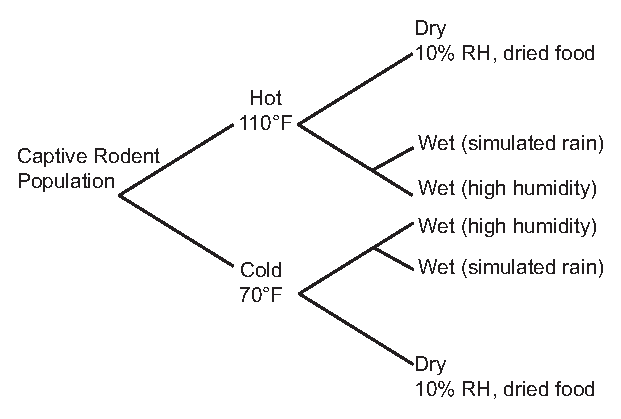
\includegraphics[width=1\textwidth]{exp_design_fig.eps}
 \end{center} 

\noindent \small{Figure 1: Animals are relegated into either hot or cold treatments. Within treatments (n=20 per treatment), animals are exposed to two weeks of varying levels of aridity, from simulated rainfall where water is available \textit{ad libitum}, to dry, where no water is available. RH=Relative Humidity}

\end{mdframed}

\vspace{5mm}


For each experiment in Aim 1, physiologic and genomic data will be collected. In the context of limited water intake, how animals achieve electrolyte balance is unknown. Electrolytes are both easy to assay and are critical to physiological well being. Indeed, proper electrolyte balance is fundamental to all other cognitive and physiological processes like neuronal signal transduction and muscle (including cardiac) contractility. Here, \ul{serum electrolytes} will be measured using the VetScan VS2 critical care panel which includes ALT, BUN, Cl, CRE, GLU, K, Na, bicarbonate ion in a 100uL sample volume. \\

In addition to assaying electrolytes themselves, measures of \ul{urine electrolytes} and \ul{osmolality} will be collected, as the urinary system represents that major pathway through which these chemicals are lost. These parameters will be measured using an Atago UG-$\alpha$ urine refractometer and tests conducted at the IDEXX reference lab. Lastly, \ul{animals will be weighed} to the nearest 0.1gm every other day, including the day of sacrifice. \ul{Body temperature} will be assayed with weighing using a digital thermometer and probe designed by World Precision Instruments (Sarasota, FL). In connection with this, \ul{feces will be collected} and water content will be measured using standard methods. \\

Key metabolic parameters such as \ul{carbon dioxide production} and \ul{oxygen consumption} that may influence water consumption will be collected. In addition, the \ul{change in relative humidity} within the metabolic chamber will be assayed, which will allow us to understand the rate of pulmonary water loss (or gain). These tests will be measured during a twenty four hour period at the end of the experimental manipulation, just prior to euthanasia, using a metabolic chamber (Sable Inc.) modified for use in the desert chamber. Together, these data will represent a uniquely rich characterization of the physiological state of a desert rodent held in captivity but more importantly, exposed to conditions typical of the natural environment. Of note, all procedures involving vertebrate animals conform to the guidelines provided in \citep{Sikes:2011dz} and have been approved by the University of New Hampshire Animal Care and Use Committee. \\

\noindent \textbf{Aim 1a:} \ul{Determine the physiologic response to drinking-water deprivation, extreme temperature, and humidity in the desert-adapted rodent \textit{P. eremicus}}. It is hypothesized that, as a result of unique mechanisms related to solute and water balance, average serum electrolyte concentrations will remain relatively constant throughout various experimental manipulations, but the variance in measured levels between individuals will increase in the most extreme conditions. These differences will be echoed in differences in urine electrolytes and concentration. Predictions regarding other parameters are detailed in Table 1. \\


Background: The human body consist of 60\% water \citep{Jequier:2009cz}. Far from a static reservoir, proper physiologic function requires water for countless processes including nutrient transport \citep{Haussinger:1996wl}, signal transduction, pH balance, thermal regulation \citep{Montain:1999ux} and the removal of metabolic waste. To accomplish these functions, approximately 2 liters of fluid are used daily - these fluids are lost mainly via the gastrointestinal and genitourinary systems, and by evaporative loss, which is accelerated greatly in extremes of heat and aridity \citep{Cheuvront:2010eg}. These losses must be matched by intake \citep{Jequier:2009cz}, mainly in the form of oral fluid intake. Though the body possesses limited reserves, when loss exceeds intake over even a short period of time, dehydration and in extreme cases, death can occur. Humans and most other animals are exquisitely sensitive to dehydration, and possess limited compensatory mechanisms, particularly when physically active. In contrast, desert rodents survive in extreme environmental conditions, often without fluid intake. Understanding the mechanisms underlying this remarkable phenotype requires we understand the physiology that accompanies it. The work described here aims to characterize the physiology of dehydration resistance in desert adapted rodents. This knowledge will allow us to understand the salient differences in renal physiology between human and desert rodent, ultimately providing a means through which therapies aimed at increasing soldier safety and performance will be developed.    \\

While the prolonged absence of drinking water is invariably fatal for humans and many other animals, one potentially mitigating effect may be the acquisition of water (or limitation of loss) via the pulmonary vasculature, which is known to be variably permeable to water \citep{Berger:2011ks,Goralski:2010eo}. While pulmonary water acquisition has not been quantified in humans or in mammalian models, the pulmonary vasculature is ideally positioned to retain water from inspired air. Following this, relative humidity -  the amount of extractable water present in respired air may be important to overall hydration status. The design described above incorporates two different levels of humidity to begin to disentangle the effects of drinking water from water acquisition via the pulmonary system. \\
\begin{wrapfigure}{r}[0pt]{.8\textwidth}
\hypertarget{Table 1}{}
\vspace{-5mm}
\begin{mdframed}
  \begin{center}
    \includegraphics[width=1\textwidth]{Aim1-table.eps}
  \end{center}
  \noindent{\small{Table 1: Predicted response given specific experimental manipulations. The number of arrows indicate the predicted relative magnitude of the response.}}
\end{mdframed}
\end{wrapfigure}

Although water stress is obviously important to the survival of desert rodents - a phenotype which is relevant to human health and wellness, extreme temperatures represent another way in which physiological processes may be challenged. While desert animals may thrive in extreme heat, humans cannot. The physiological response is characterized in model organisms, but not in other animals adapted to these conditions. Genes like the heat-shock proteins are protective in humans, but no record of their activity on desert rodents is known. \\

Research Plan: To accomplish this aim, physiologic data from animals held with and without drinking water will be gathered, factorial with respect to the other conditions (e.g. temperature and humidity). The specific experiments described in \hypertarget{Figure 1}{Figure 1} will allow us to tease apart the effects of water deprivation from other parameters. Though the data we propose to collect is described above, in brief, we plan to collect blood and urine electrolytes and urine specific gravity. We will collect data on fecal water content, animal weight and temperature, as well as a battery of metabolic parameters. The specific predictions regarding several of these parameters are described in Table 1.  \\

The statistical treatment of the data will include a multivariate regression to establish the relationships between the genomic and physiologic data. Many of these analyses will be conducted with non-parametric tests, as data are often non-normally distributed nor independent. One of the most interesting comparisons will be to understand the relationship between serum sodium and urine sodium, urine concentration, fecal water content, and changes in body weight. Ultimately (e.g. Aim 1b) these data will be linked with patterns of gene expression, methylation, and isoform use to gain a synthetic understanding of dehydration resistance. \\




% \begin{center}
%  \includegraphics[width=.5\textwidth]{Aim1-table.eps}
% \end{center} 
%
%\noindent \small{Table 1: Say something about predictions here.}
%
%\vspace{4mm}


Preliminary data: The electrolyte profile of 5 individuals housed at 70F, 50\% RH, water \textit{ad lib} and two individuals housed in identical conditions except that drinking water was withheld has been characterized. Despite being housed in typical laboratory conditions, these animals have remarkably unusual electrolyte panel. For instance, mean serum sodium is 152 mmol/L, chloride 105 mmol/L, potassium in an un-hemolyzed sample is unusually high by human standards at 8.1 mmol/L, while Creatinine is low, with a mean measurement of 0.25mg/dL. mean blood urea nitrogen (BUN) is 47mg/dL. In contrast, animals without \textit{ad lib} water were obviously dehydrated, with a mean serum sodium of \textgreater 170 mmol/L and chloride 126 mmol/L. Interesting severe dehydration was not complicated by renal impairment as evidenced by a mean serum creatinine of 0.3 mg/dL and BUN of 59 mg/dL. Animals lost a remarkable amount of weight, on average 28\% of total body weight. Despite this decline in weight and electrolyte derangement, animals were active as per usual. \textbf{These results are shockingly distinct from human response to dehydration, and warrant further study.}  \\  

\noindent \textbf{Aim 1b:} \ul{Define patterns of gene expression, isoform use, and methylation given differences in environmental condition}. {We will understand the genetic response to extreme heat and aridity via a series of Illumina bisulfite and mRNA sequencing, and PacBio sequencing experiments, and will link these patterns to individual physiologic state as defined in Aim 1.} We hypothesize that genes responsible for water and solute transport will be particularly active in the most extreme conditions in renal and pulmonary tissues, while genes involved in the activation of the hypothalamic-neurohypophysial system will be differentially regulated in the hypothalamus. The genes identified here will provide the requisite foundation on which interventions aimed at increasing soldier safety and performance will be developed. \\

Background: Broadly speaking, genes underlie the vast majority of observable phenotypes. Whether this relationship is mediated by patterns of expression (e.g. \cite{Teets:2012gt}), which itself may be mediated by differences in methylation \citep{Brenet:2011dq}, or by use of alternative splice isoforms \citep{Yukutake:2010ia}, linking genotype to phenotype is extremely difficult. In addition to these mechanisms, function (=phenotype) may be determined by post-translational modifications like phosphorylation of specific sites \citep{Anonymous:2009gb}. The identification of these mechanisms is important, not only because in doing so we gain a deeper understanding of evolution, but also because these molecular mechanisms may be later used as targets for drug development or other therapeutic intervention. With regards to resistance to dehydration, the development of novel interventions is critical, as tens of thousands of troops serve in arid areas - each one of them threatened daily by the dehydration-related decline in physical and cognitive performance. \\

In model organisms, dehydration precipitates a physiological response that is largely driven by the neuroendocrine system. Very much simplified, the cascade begins with the stimulation of osmoreceptors \citep{Arsenijevic:1985bi}, which in turn stimulates neurons located in the paraventricular and supraoptic nuclei of the hypothalamus to release anti-diuretic hormone (ADH) \citep{Zingg:1986vb}. ADH then binds to vasopressin-responsive receptors located in the renal medulla, resulting in aquaporin movement to the surface of the collecting duct \citep{Nielsen:1995uq} which encourages water re-uptake. In addition to the aquaporins, the renin-angiotensin-aldosterone system \citep{Gubler:2010bh}, natriuretic peptides \citep{Totsune:1994kf}, the SLC and mTOR families \citep{Ortells:2012go}, and potentially other yet to be discovered pathways are important to water balance. Far from canonical, each stage in these cascades is dynamic and therefore pathways revealed in \textit{Mus} and humans may not be equivalent to pathways in uniquely adapted desert animals, particularly given radically different phenotypes. Understanding these mechanisms is critical to the development of interventions. \\

The genomic processes related to dehydration resistance in desert animals has yet to be characterized. The few studies of genetics that have been conducted have focused on the role of expression of single members of the aquaporin gene family (but see \cite{Bartolo:2007hy}), which are large membrane-bound proteins that are critically involved in renal water transport \citep{Kwon:2009bv,Verkman:2002ww,Brown:1995vo,Nielsen:1995cb}. These studies have shown that changes in Aquaporin (AQP) protein abundance and expression may be related to water availability \citep{Boselt:2009fb, Gallardo:2005fm,Bozinovic:2003eg}. In addition to changes in expression, another study showed that the AQP4 pathway was completely lost in the desert rodent \textit{Dipodomys merriami merriami} \citep{Huang:2001ti}. Despite these studies, we have a limited understanding of the genomics of renal water and solute regulation in desert animals. While AQPs are functionally important, water and solute balance is extraordinarily complex, and therefore single-gene studies are necessarily limited in their purview. A more complete understanding of this phenotype and its mechanistic underpinnings will require a sophisticated genome-level approach, which will be the outcome of the proposed research. In contrast to the limited amount known about patterns of renal gene expression, much less is known about gene expression in other tissues, and absolutely nothing about differential methylation or isoform use, even though we know that these complexities are mechanistically important to this specific function \citep{Yukutake:2010ia,Silberstein:2004ex}. \\

Research Plan: The analysis of the genome wide patterns of response to dehydration will be conducted using the same individuals for which we collected physiology data. To accomplish this goal, RNAseq libraries for each individual and tissue (n=120 animals * 3 tissues) will be constructed. Sequencing will be conducted at the New York Genome Center on a HiSeq 2500. We aim to generate approximately 20-30 million 125nt paired-end sequences per sample, which corresponds to 36 high-output HiSeq lanes using 10-way multiplexing. \\ 

RNAseq reads derived from kidney, lung, and hypothalamus will be mapped to the existing annotated draft genome, which was sequenced using startup funds. This phase of the project will be accomplished using the short read aligner BWA \citep{Li:2013wn} and best practices previously established \citep{MacManes:2014io}. Differential expression will be evaluated via the Cufflinks package \citep{Trapnell:2012kp}, while evidence for coordinated changes in large numbers of genes will be detected using the software wcgna \citep{Langfelder:2008bd}. The MacManes lab has demonstrated expertise in this area.\\

Accurate isoform reconstruction is notoriously difficult using high-throughput short read sequence data such as that produced by Illumina HiSeq platform \citep{Pyrkosz:2013tm,Hiller:2009be}, despite the advent of longer read lengths and newer analytical techniques \citep{LeGault:2013gw,Jiang:2009bw}. In projects like this, where differential isoform use may be critical to phenotype, a different approach may be warranted. For instance, the sequencing technology available from Pacific Biosystems (PacBio) is suggested to provide a resolution to the isoform reconstruction problems \citep{Au:2013hp}, specifically because it involves a long-read single molecule sequencing strategy \citep{Eid:2009kva}.  To identify patterns of differential isoform use, we will sequence poly-A selected mRNA samples using PacBio technology. Reads will be error corrected using the program LSC \citep{Au:2012iq}, and isoforms will be identified using methods contained in \cite{Au:2013hp}. Because PacBio throughput is relatively low, which may limit the precision with which quantitation can be achieved, we will explore alternative ways to accurately estimate isoform specific expression. One previously unexplored approach involves estimating expression in the program eXpress \citep{Roberts:2012dh} using only those reads that map uniquely and unambiguously to a specific isoform. Because this approach is uncharacterized, it will be validated using a set of isoform specific qPCR primers that will allow us to estimate isoform-specific expression using digital PCR.  \\ 

Lastly, aside from differences in expression of isoform use, patterns of methylation could be important in the development of extreme osmoregulation - indeed, methylation has been shown to be important to many other complex phenotypes including behavior \citep{Lyko:2010dr}, metabolism \citep{Foret:2012jf}, and physiologic stress (including heat stress) response \citep{Sonna:2002dc}. To understand patterns of methylation, a large bisulfite sequence dataset will be generated, which will contain information from every individual included in the mRNAseq experiments, described above. This dataset will allow for the understanding of another layer of genomic complexity not typically available to researchers conducting RNAseq experiments in isolation. Importantly, in addition to enhancing our understanding of the mechanisms underlying dehydration tolerance, phenotypes related to differential methylation may be prime therapeutic targets.    \\


%\begin{wrapfigure}{l}[0pt]{0.6\textwidth}
%\hypertarget{Table 1}{}
%\vspace{-5mm}
%\begin{mdframed}
%  \begin{center}
%    \includegraphics[width=1\textwidth]{Aim1-table.eps}
%  \end{center}
%  \noindent{\small{Table 1: Say something about predictions here.}}
%\end{mdframed}
%\end{wrapfigure}


Preliminary Data: To date, the lab has generated a RNAseq dataset that consists of approximately 30M 150nt SE Illumina reads from the same 5 animals housed in the 'cold/simulated rain' treatment group from which physiology data was collected. We have generated \textit{de novo} transcriptome assemblies as well as mapped to the reference genome. Though the scope of the analyses is preliminary, the results are interesting. 99.7\% of the RNAseq reads map to the genome, with over 73\% mapping concordantly. This suggests that the content of the draft genome is compete and genic contiguity is high. We have recovered many of the aquaporin genes, as well as many other critical genes including vasopressin and its receptor, Renin, Angiotensin, Angiotensin Converting Enzyme, as well as the genes that code for the natriuretic peptides. We have estimated expression for all transcripts.  Interestingly, within the aquaporin genes, Aquaporins 1 and 2 had the highest expression, while expression of Aquaporin 5, 9, 10 and 12 were undetectable, though they are present in the genomic reference.  \\

\hypertarget{Table 1}{}
\vspace{-5mm}
\begin{mdframed}
  \begin{center}
    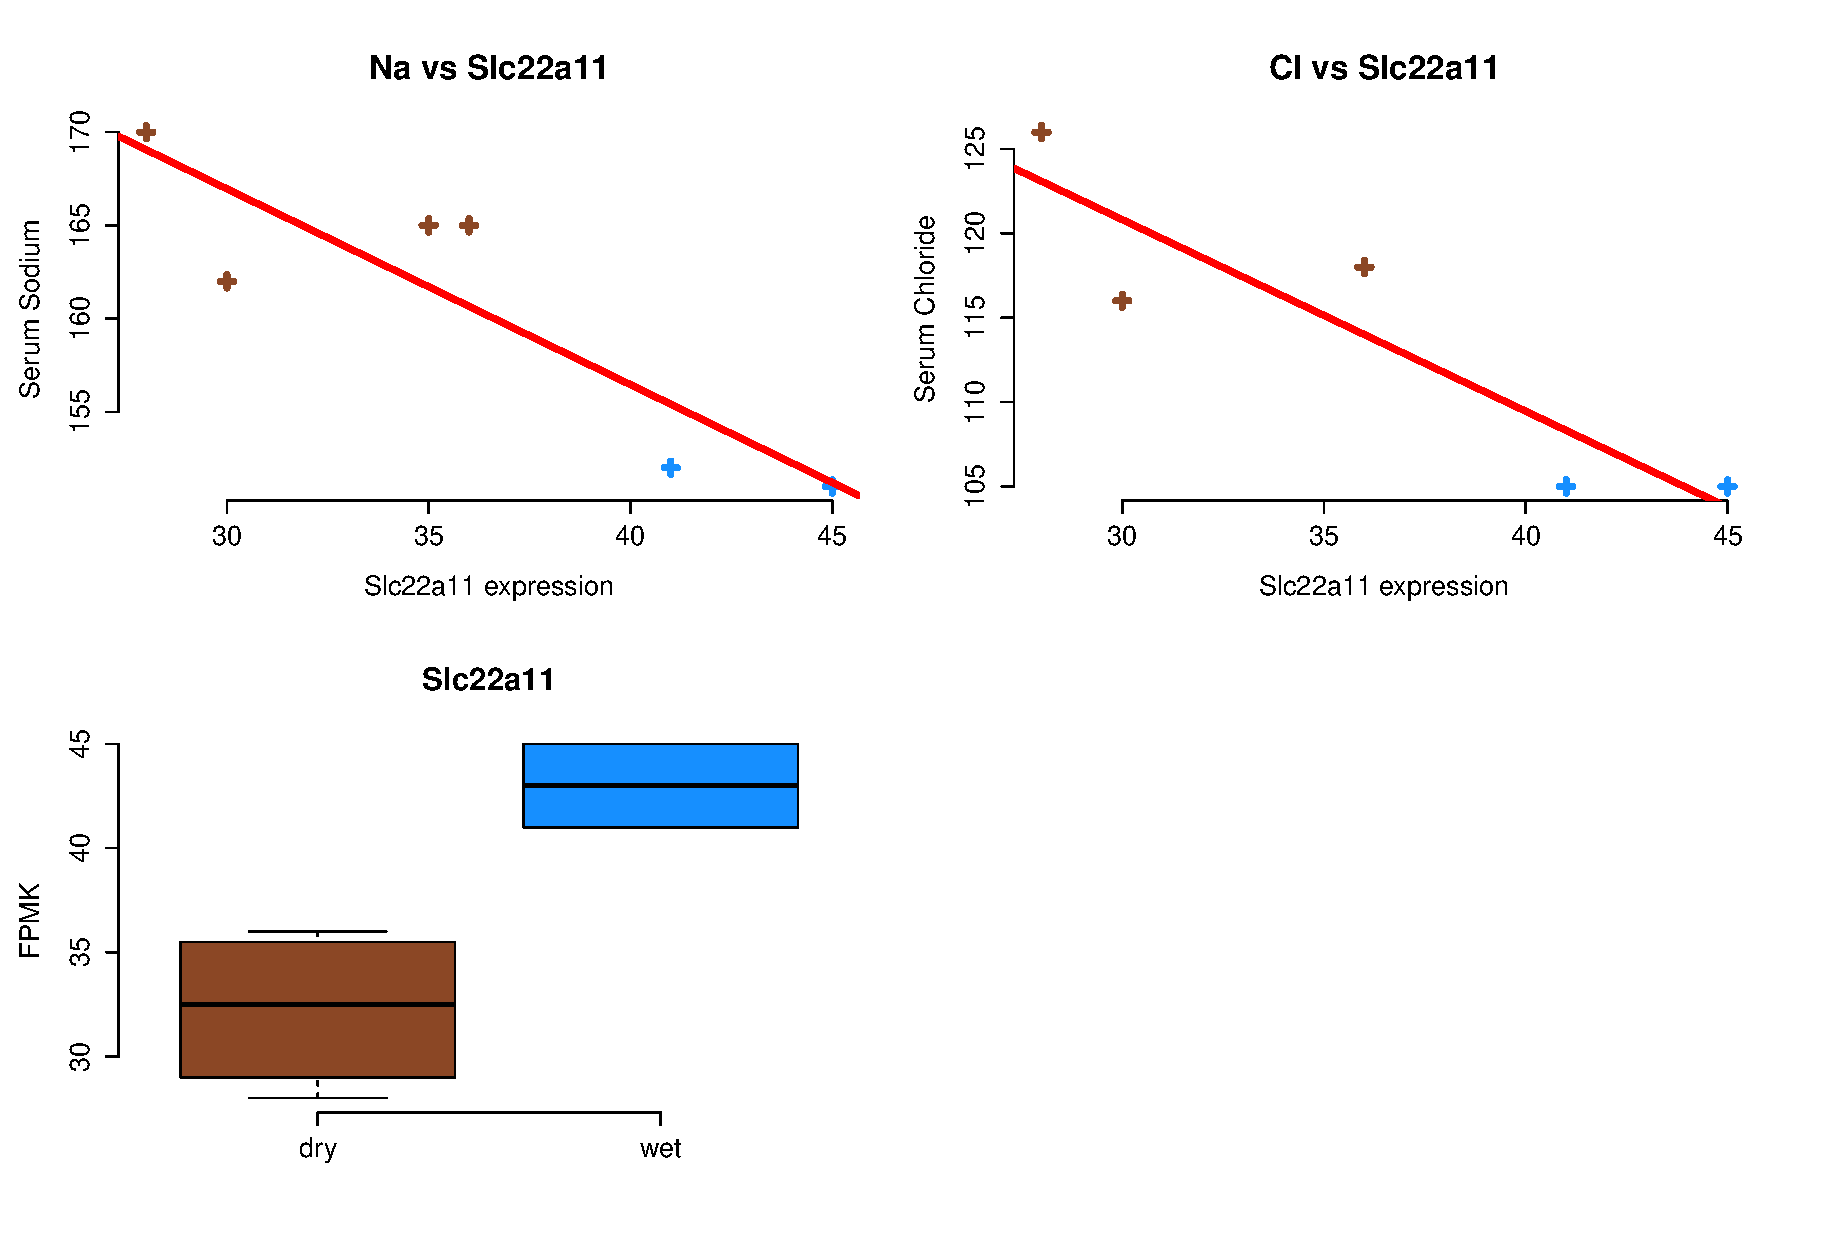
\includegraphics[width=1\textwidth]{slc.eps}
  \end{center}
  \vspace{-5mm}
  \noindent{\small{Figure 2: The solute carrier gene Slc22a11 is significantly differentially expressed between dehydrated (represented by brown color) and hydrated (blue color) mice. Additionally, the gene is strongly related to both serum Sodium and Chloride ions.}}
\end{mdframed}


Testing for differential gene expression between the hydrated and dehydrated mice though preliminary, were extremely interesting. While we had the \textit{a priori} expectation that the aquaporins would be differentially expressed, many of the solute carrier (SLC) and ion transport genes were significantly unregulated dehydrated mice. Figure 2 illustrate this patters, with Slc22a11, a cation/anion transporter \citep{Koepsell:2004kg}, significantly differentially expressed and related to serum Sodium and Chloride concentrations. This suggests a possible compensatory mechanism, especially exciting as solute carriers have recently emerged as novel drug targets \citep{RaskAndersen:2013cu}. Together, the biological results coupled with increasing interest from pharma suggests that the development of strategies aimed at enhancing soldier safety and performance my ultimately be possible.  


Expected Outcome: Upon completion of Aim 1, we will have a synthetic understanding of the physiologic and genomics patterns associated with extreme osmoregulation required for survival in desert environments. These data will allow us to generate a list of genes, genomic regions, isoforms, and methylation states putatively linked to the phenotype of interest. This list is critical, and will form the basis for future applied work, which will propose the development of a system where manipulation of specific genes is possible (e.g. the CRISPR/CAS9 transgenic system or via inhibitory medicines), thus moving the work from correlation to causation. Ultimately, we envision partnering with experts in drug development and delivery to bring these interventions to humans - here specifically with the goal of enhancing soldier safety and performance specifically in desert environments. \\

\noindent \textbf{Aim 2:} \ul{Given the transition from the obligate intake of fluids as infants, to it’s complete absence later in life, the ontogeny of physiologic water conservation will be elucidated.} \\

Background: Given that desert adapted mice, capable of surviving without water are as neonates dependent on liquid intake, {the study of the ontogeny of physiologic water conservation is extremely interesting and relevant to the current work.} The study of gene expression in renal, pulmonary and hypothalamus tissue types along the transition from the intrauterine environment through birth in the context of differences in oral fluid intake is remarkably novel and will yield unique insights into physiologic water conservation. Although several studies have assayed renal gene expression in neonates, these studies have typically been limited to a small number of genes in a specific context (e.g. studies of hypertension \citep{Sampson:2012hb,Shanmugam:1996ed}). The proposed work aims to leverage this unique developmental stage to uncover genes underlying this transition. While the physiology of neonates is clearly different from that of soldiers working in desert environments, gaining an understanding of the mechanisms underlying this developmental transition from \textit{ad libitum} water intake to a compete absence will directly inform our understanding. This aim may wholly reinforce the findings of aim 1, or suggest completely different pathways; both outcomes clearly enhancing the overarching goals of the research project. \\

In addition to the transition from lactation-dependence through weaning, an even more fundamental transition happens at birth, which is accompanied by substantial changes in renal physiology. In utero, the large volumes of dilute urine are typically produced \citep{Wintour:1997ts} while post-birth, relatively small volumes of concentrated urine are typical. While this trend appears to be canonical in well-characterized mammal models, whether the fetuses of water-stressed desert-adapted mice follow this trend is unknown, and may be extremely revealing in the context of dehydration resistance. The proposed work aims to use a genome wide approach to characterize these transitions in desert-adapted rodents. This work will provide novel insights into fundamental biological processes, bearing hard upon dehydration resistance which is directly relevant to the explicit goals of this project.   \\  

Research Plan: This phenomenon will be explored using fetal and neonatal mice whose mothers are exposed to treatments and an abbreviated set of methods listed in Aim 1. Many of the physiological measurements  (e.g. blood and urine analyses) will be impossible to collect in very young animals secondary to sample volume requirements, though a full battery of genomic tests will be possible. To evaluate the ontogeny, five fetal and neonatal mice will be culled per treatment at four different time-points (immediately prior to birth, 2 hours after birth, mid-lactation (approximately 10 days after birth), 1 day after weaning). These time-points have been chosen as together they will allow us to assay the breadth of developmental stages.  We hypothesize that patterns of gene expression, methylation, and isoform use will resemble those common in conditions where water is available \textit{ad lib}, though the novelty of this aspect of the study limits firm predictions. \\

Expected Outcome: Upon completion of Aim 2, we will have a synthetic understanding of the genomics patterns associated with the ontogeny of extreme osmoregulation. These data, together with the data associated with Aim 1 will allow us to generate a list of genes, genomic regions, isoforms, and methylation states putatively linked to the phenotype of interest. This list is critical, and will form the basis for future applied work, which will propose the development of a system where manipulation of specific genes is possible (e.g. the CRISPR/CAS9 transgenic system or via inhibitory medicines), thus moving the work from correlation to causation. Ultimately, we envision partnering with experts in drug development and delivery to bring these interventions to humans - here specifically with the goal of enhancing soldier safety and performance specifically in desert environments.  \\



\noindent \textbf{CONCLUSIONS} \\

Soldiers serving in desert environments are forced to endure intense heat and aridity inherent to these environments. Indeed, these environmental stressors represent a real threat to the health and performance of these individuals. While humans are generally ill-suited to perform in these environments other mammals, specifically those having evolved in deserts are extremely well adapted. In particular, many desert mammals may survive without water intake. Understanding the physiology and genetics of this remarkable ability will provide the critical 1$^{st}$ steps toward enhancing soldier safety and performance in desert environments by reducing the requirements for oral fluid intake. This basic science research proposal aims to understand the physiology, genetic and genomic underpinnings of survival without water in a desert-adapted rodent native to the Southwest United States, \textit{Peromyscus eremicus}. Our long-term goal includes developing the ability to recapitulate the phenotype in non-desert adapted mammals, including humans.


\vspace{3mm}
\textbf{Table 2: Timeline}
\hypertarget{Table 2}{}
\begin{center}
\begin{tabular}{l|c c r}

\textsc{Activity} & \textsc{FY2015} & \textsc{FY2016} & \textsc{FY2017} \\
\hline \\
\textsc{Increase Colony Size \& ID animals for experiments } & X & & \\
\textsc{Conduct Physiology Experiments -- AIM 1A} & X & & \\
\textsc{Collect \& Analyze expression data -- AIM 1B} & X & & \\
\textsc{Analyze Bisulfite and PacBio data -- AIM 1B} & & X & \\
\textsc{} & &  &   \\
\textsc{Animal breeding in prep for Aim 2} & & X &  \\
\textsc{Collect \& Analyze genomic data -- AIM 2} & & X & X \\
\textsc{} & &  &   \\
\textsc{Write papers} & & X & X \\
\textsc{Present results at international conference} & & X & X \\
\textsc{Prepare grant aimed at funding applied research} & & X & X \\
\textsc{Train Undergrad, Grad students} & X & X & X \\
\textsc{Disseminate info} & X & X & X \\

\end{tabular}
\end{center}
\vspace{5mm}

\newpage
%\setcounter{page}{1}
%\thispagestyle{empty}
\singlespacing
\bibliographystyle{model2-names-edit.bst}

\bibliography{/Users/macmanes/Documents/army/biblio.bib}


































\end{document}
